% Created 2021-09-12 Sun 22:49
% Intended LaTeX compiler: xelatex
\documentclass[letterpaper]{article}
\usepackage{graphicx}
\usepackage{grffile}
\usepackage{longtable}
\usepackage{wrapfig}
\usepackage{rotating}
\usepackage[normalem]{ulem}
\usepackage{amsmath}
\usepackage{textcomp}
\usepackage{amssymb}
\usepackage{capt-of}
\usepackage{hyperref}
\usepackage[margin=1in]{geometry}
\usepackage{fontspec}
\usepackage{indentfirst}
\setmainfont[ItalicFont = LiberationSans-Italic, BoldFont = LiberationSans-Bold, BoldItalicFont = LiberationSans-BoldItalic]{LiberationSans}
\newfontfamily\NHLight[ItalicFont = LiberationSansNarrow-Italic, BoldFont       = LiberationSansNarrow-Bold, BoldItalicFont = LiberationSansNarrow-BoldItalic]{LiberationSansNarrow}
\newcommand\textrmlf[1]{{\NHLight#1}}
\newcommand\textitlf[1]{{\NHLight\itshape#1}}
\let\textbflf\textrm
\newcommand\textulf[1]{{\NHLight\bfseries#1}}
\newcommand\textuitlf[1]{{\NHLight\bfseries\itshape#1}}
\usepackage{fancyhdr}
\pagestyle{fancy}
\usepackage{titlesec}
\usepackage{titling}
\makeatletter
\lhead{\textbf{\@title}}
\makeatother
\rhead{\textrmlf{Compiled} \today}
\lfoot{\theauthor\ \textbullet \ \textbf{2021-2022}}
\cfoot{}
\rfoot{\textrmlf{Page} \thepage}
\titleformat{\section} {\Large} {\textrmlf{\thesection} {|}} {0.3em} {\textbf}
\titleformat{\subsection} {\large} {\textrmlf{\thesubsection} {|}} {0.2em} {\textbf}
\titleformat{\subsubsection} {\large} {\textrmlf{\thesubsubsection} {|}} {0.1em} {\textbf}
\setlength{\parskip}{0.45em}
\renewcommand\maketitle{}
\author{Houjun Liu, Exr0n}
\date{\today}
\title{Heart of Darkness (index)}
\hypersetup{
 pdfauthor={Houjun Liu, Exr0n},
 pdftitle={Heart of Darkness (index)},
 pdfkeywords={},
 pdfsubject={},
 pdfcreator={Emacs 28.0.50 (Org mode 9.4.4)}, 
 pdflang={English}}
\begin{document}

\maketitle


\section{Heart of Darkness}
\label{sec:orga810a53}
Not the Heart of Hardness.

\href{https://docs.google.com/presentation/d/1a9mxL5Pot8sbcIYP1mLiFqhQrYEOa60eIyHp3ftTLGo}{Alexa
and Nueva folks, the Slides.}

Ok. Now that that's out of the way, let's deal with this "Bloody Racist"
book. To understand this work fully, one must understand Congo, its
govermental systems, and the Scramble for Africa (Africa's cakeification
by Europeans).

\subsection{About the Author}
\label{sec:orgd3c46d4}
\begin{itemize}
\item Born in conquered location
\item wrote HoD in english (not native tougue)
\item became a sailor
\end{itemize}

\subsection{Scramble for africa}
\label{sec:orge998b8d}
\begin{itemize}
\item Europe goes after things in africa

\begin{itemize}
\item ivory
\item gold
\item labor
\item diamonds
\item land
\item food
\item rubber
\end{itemize}

\item \href{https://www.youtube.com/watch?v=EKE92ucqBfc}{Visualization} \#\#\# The
Slave Trade
\item Taken away:

\begin{itemize}
\item Male, 13-43
\item Woman
\item Children
\item Left behind: babies and elderly
\end{itemize}

\item Effects

\begin{itemize}
\item Population drops
\item No more labor force
\end{itemize}

\item non diverse economy
\item colonized countries are dependant on the empire
\item lack of infrastructure
\item discrimination and racism
\end{itemize}

\subsubsection{Presense in Africa}
\label{sec:org21c71c7}
\begin{itemize}
\item Biggest colonies: france and england \#\#\#\# Started on the coast
\item Because they needed steamships and quinine (tonic water) to go into
the center
\end{itemize}

\subsubsection{Naming: heart of darkness}
\label{sec:org0c33239}
\begin{itemize}
\item Civilization
\item Skin color
\end{itemize}

\subsubsection{Berlin Congress}
\label{sec:orgacfdcf5}
\begin{itemize}
\item Countries got together and divied up africa amongst themselves
\end{itemize}

\subsubsection{Congo Free State}
\label{sec:org01f2a70}
\begin{itemize}
\item King leopold II believed that a country needed a colony to be cool

\begin{itemize}
\item created international association of the congo
\item promised to promote humanitarian things
\item "skillful and cunnnin diplomacy"
\item slash vines for rubber and get it on yourself then scrape it off

\begin{itemize}
\item this kills the vines which means you have to keep moving
\item rubber used for bikes and cars
\item Pay tax or get mutilated / killed
\end{itemize}

\item \href{https://www.youtube.com/watch?v=FhPZZqp9cp8}{Humanitarian
atrocities videos} \#\#\#
\href{http://loki.stockton.edu/\~kinsellt/projects/hod/history.html}{History
of Congo Region}
\end{itemize}
\end{itemize}

\subsection{Critical Theory}
\label{sec:org1c807f8}
An approach to contentualize a text + see through to something. Think:
"a feminist lens" --- Critical Race Theory, Queer Theory, Maxist Theory,
Feminist Theory, Post-Colonial Theory, Colonial Theory, Cultral Studies,
etc. etc.

And, here's the rub: \textbf{History is Written by the Victors} --- an
important part of the analysis of the \emph{Heart of Darkness} is to
recognize its story in a Colonial Lens.

\href{https://owl.purdue.edu/owl/subject\_specific\_writing/writing\_in\_literature/literary\_theory\_and\_schools\_of\_criticism/}{The
Various Lit Theories}

\subsubsection{Colonial Theory}
\label{sec:org8334b56}
\begin{itemize}
\item View through the Colonizer
\item "Written by the victors"
\end{itemize}

\subsection{Congo's Colonial History}
\label{sec:org7d61410}
\subsubsection{A timeline!}
\label{sec:orgcd7d342}
\begin{figure}[htbp]
\centering
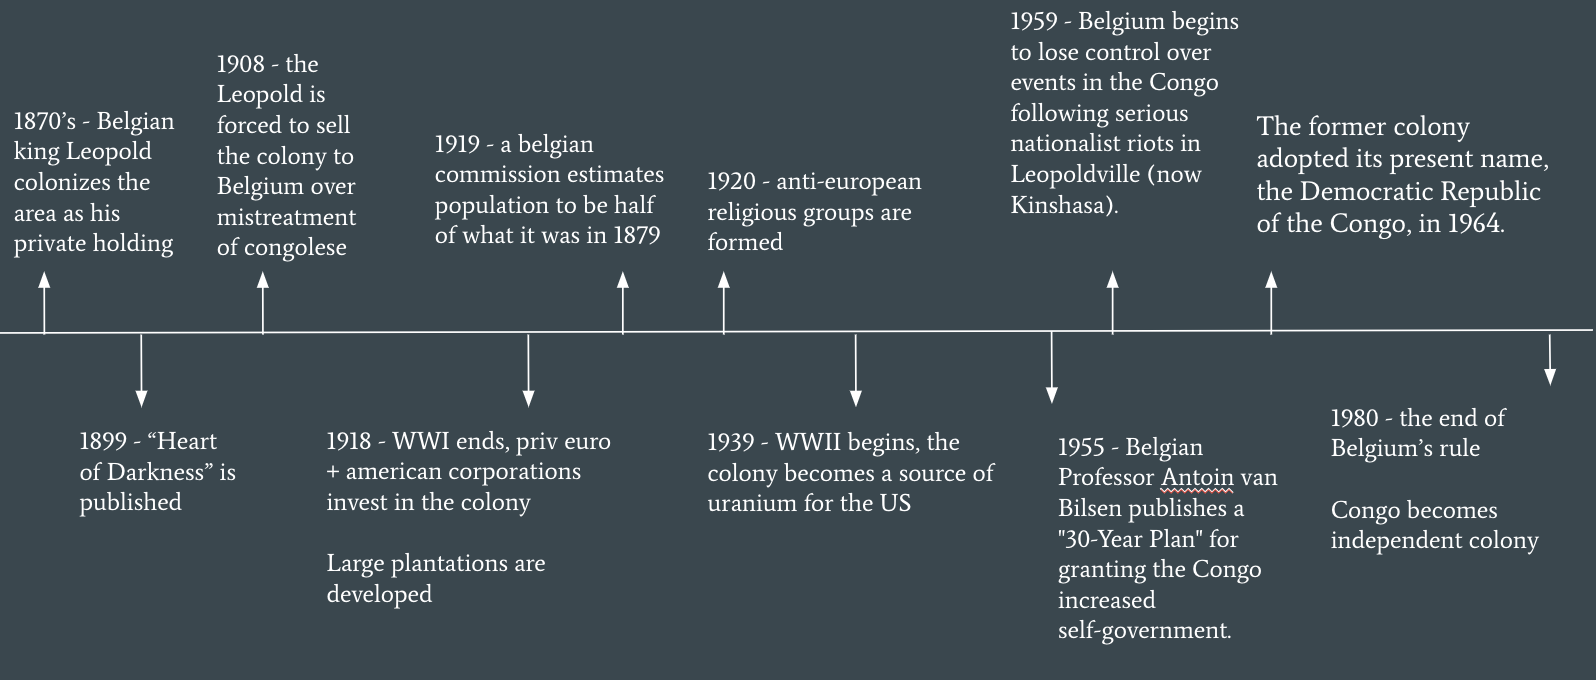
\includegraphics[width=.9\linewidth]{Screen Shot 2020-09-08 at 2.00.47 PM.png}
\caption{Timeline}
\end{figure}

\subsubsection{Some background on the Congo Free State}
\label{sec:org9478f02}
The \href{KBhENG201CongoFreeState.org}{KBhENG201CongoFreeState}

\subsection{Reflections}
\label{sec:org0c95052}
\href{KBhENG201Page0t17.org}{KBhENG201Page0t17}
\href{KBe20eng201part1.org}{KBe20eng201part1}

\subsection{Why are we reading it?}
\label{sec:org98058aa}
For answers to the essential question, of course!
\href{KBhENG201AlexaD1.org}{KBhENG201AlexaD1}

\begin{itemize}
\item How do literature, language, and storytelling both perpetuate and
dismantle the tools of the colonizer?

\begin{itemize}
\item Could be a text that attempts to dismatle racism => "loot at the
damage that Europeans did"
\item Could be a text that attempts to propergate racism
\end{itemize}

\item How does colonialism shift notions of race, equity, socio-economic
status, natural resources, religion for the colonizer, colonized, and
the reader?
\end{itemize}

\subsection{Objectives}
\label{sec:org8afcd81}
\textbf{Central to Know}

\begin{itemize}
\item Basics of plot and character development

\item Conrad's style and key lit devices

\item History of colonialism in Africa

\item King Leopold took "Ethiopia", and sectioned it off

\item Spain and Portugal agreement => "spain has Americas, protugal has
africa"
\end{itemize}

\textbf{Important to Know}

\begin{itemize}
\item Engagement with Essential Questions
\item Conrad's background
\end{itemize}

\textbf{Nice to Know}

\begin{itemize}
\item Modernism + Heart of Darkness's relationship to lit history
\end{itemize}

\noindent\rule{\textwidth}{0.5pt}

*"The sunken eyes looked up \ldots{} vacant \ldots{} a kind of blind, white
flicker in the depths of the orbs, which died out slowly. \ldots{} I found
nothing else \ldots{} but to offer him \ldots{} biscuits. The fingers closed
slowly on it and held --- there was no other movement and no other
glance."*

"Deadness in the eyes" => \{the soul, the witness, sense, knowledge\} =>
"the fool is blind"

\begin{itemize}
\item His eyes => the sunken eyes
\item His fingers => the fingers
\end{itemize}

Ambiguity and dehumanization of fingers

\begin{itemize}
\item Frequent talk about the feature
\item No descriptions as a whole
\item Description of the \emph{non-black} parts of the body only

\begin{itemize}
\item Notices and grapples with the darkness
\item "White Eyes, Hands, etc" => notices the whiteness
\item Dehumanization
\end{itemize}

\item Porchugal invented a faster boat
\item Brits and Franchies and Dutch had more nefarious goal
\end{itemize}

\subsection{Graded Discussion}
\label{sec:orge26f6dd}
\href{KBENG201GradedDiscussionPrep.org}{KBENG201GradedDiscussionPrep}

\subsection{Essays}
\label{sec:org02fec6d}
M.A. HoD Lit Analysis

\begin{itemize}
\item Jack's Take:
\href{KBENG201HoDLitAnalysisEssay.org}{KBENG201HoDLitAnalysisEssay}
\end{itemize}
\end{document}
